\section{Parallel Tempering in a nutshell}

\begin{figure}[t]
  \centering
    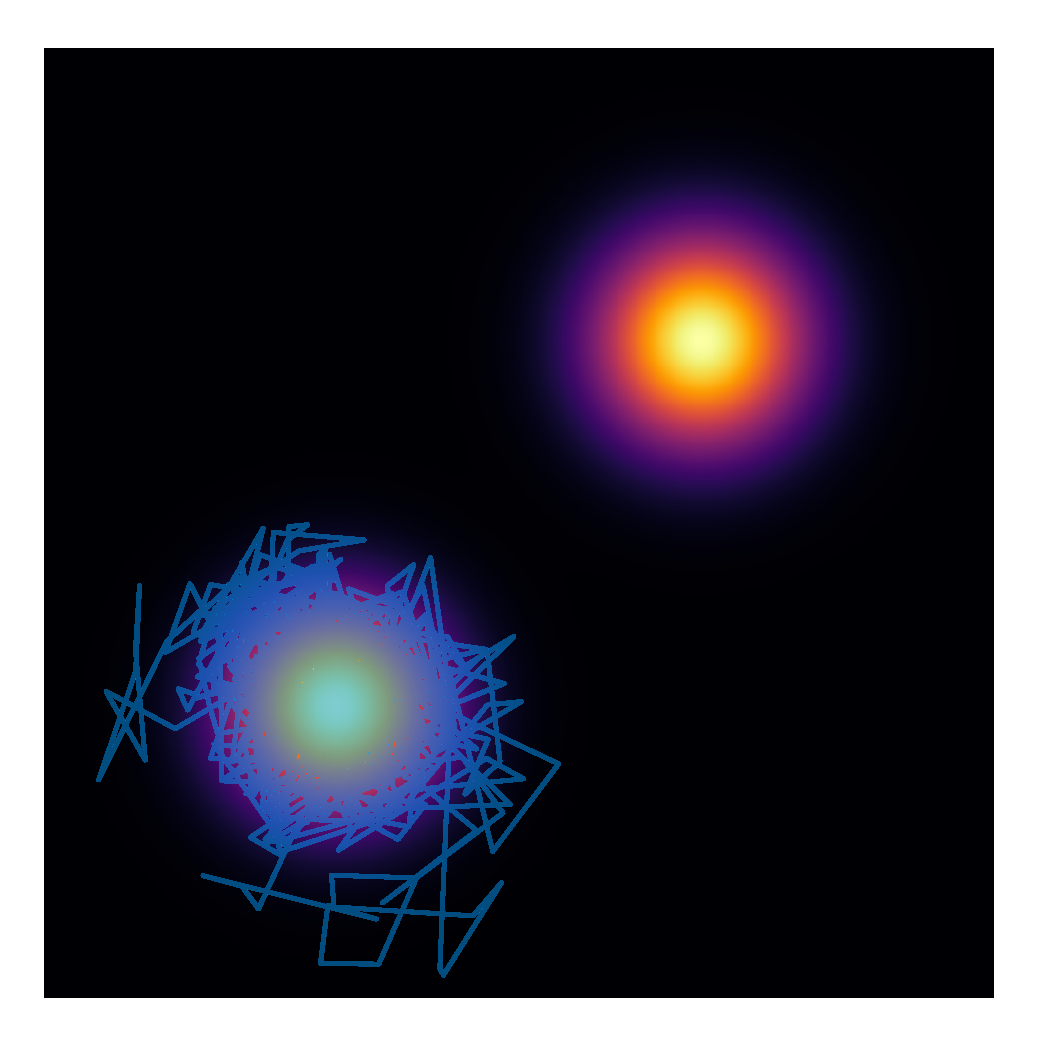
\includegraphics[width=0.5\linewidth]{../img/bimodal.pdf}
    \caption{A bimodal distribution. Blue lines display output 
    from 1,000 iterations of a random walk Metropolis-Hastings sampler.}
    \label{fig:bimodal}
\end{figure}

Consider the problem of sampling from a probability density (or mass) function
$\pi(x)$, henceforth called the \emph{target}. Solving this task is often 
challenging, as the 
distribution $\pi$ can exhibit features which traditional MCMC methods---from
random walk Metropolis-Hastings to Hamiltonian Monte Carlo---struggle to
describe accurately. For example, in bimodal distributions such as the one 
illustrated in \cref{fig:bimodal}, traditional methods might remain stuck in one 
of the two modes for an extremely long period of time.

\begin{figure}[t]
  \centering
    \begin{minipage}{0.333\linewidth}
      \centering
      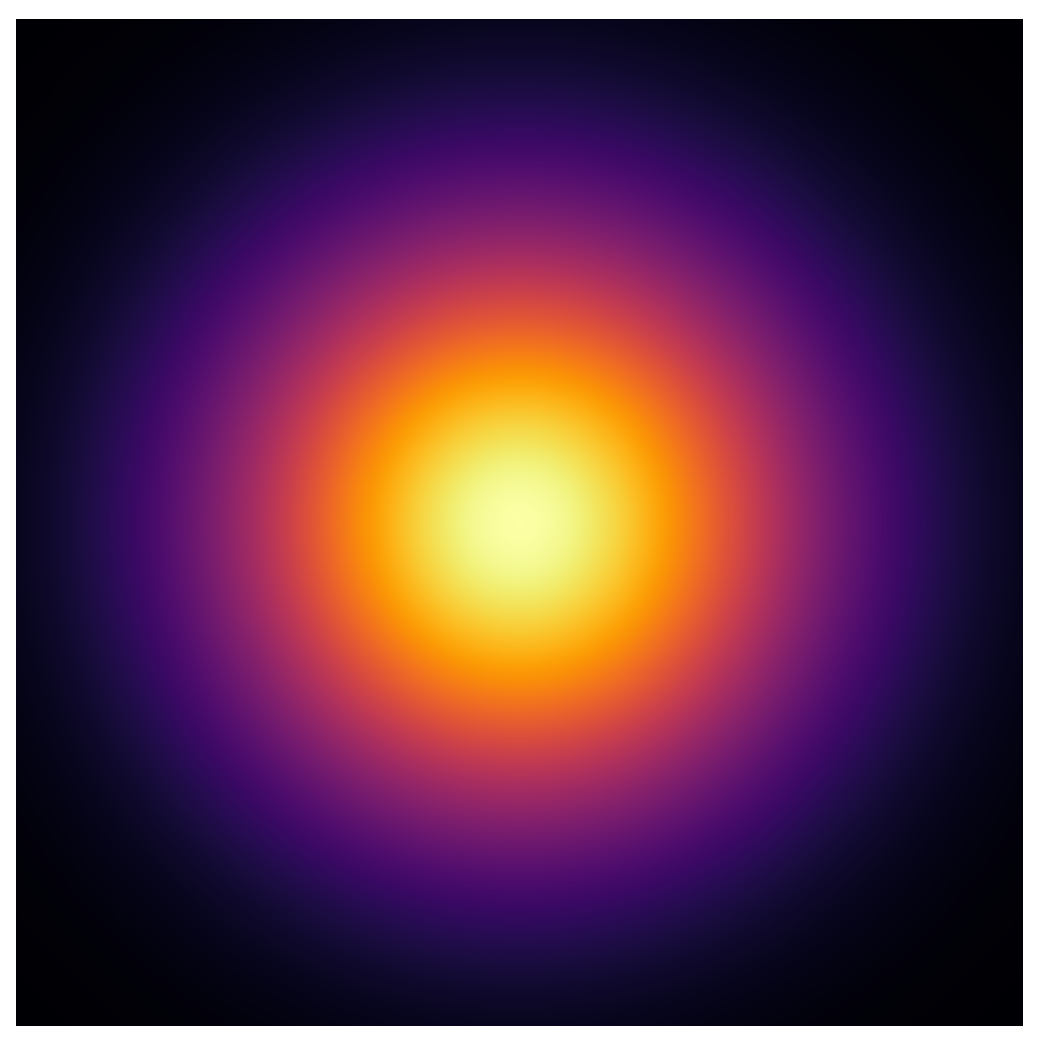
\includegraphics[width=\linewidth]{../img/heatmap_path_1.pdf}
%      \caption*{$\pi_1$}
    \end{minipage}%
    \begin{minipage}{0.333\linewidth}
      \centering
      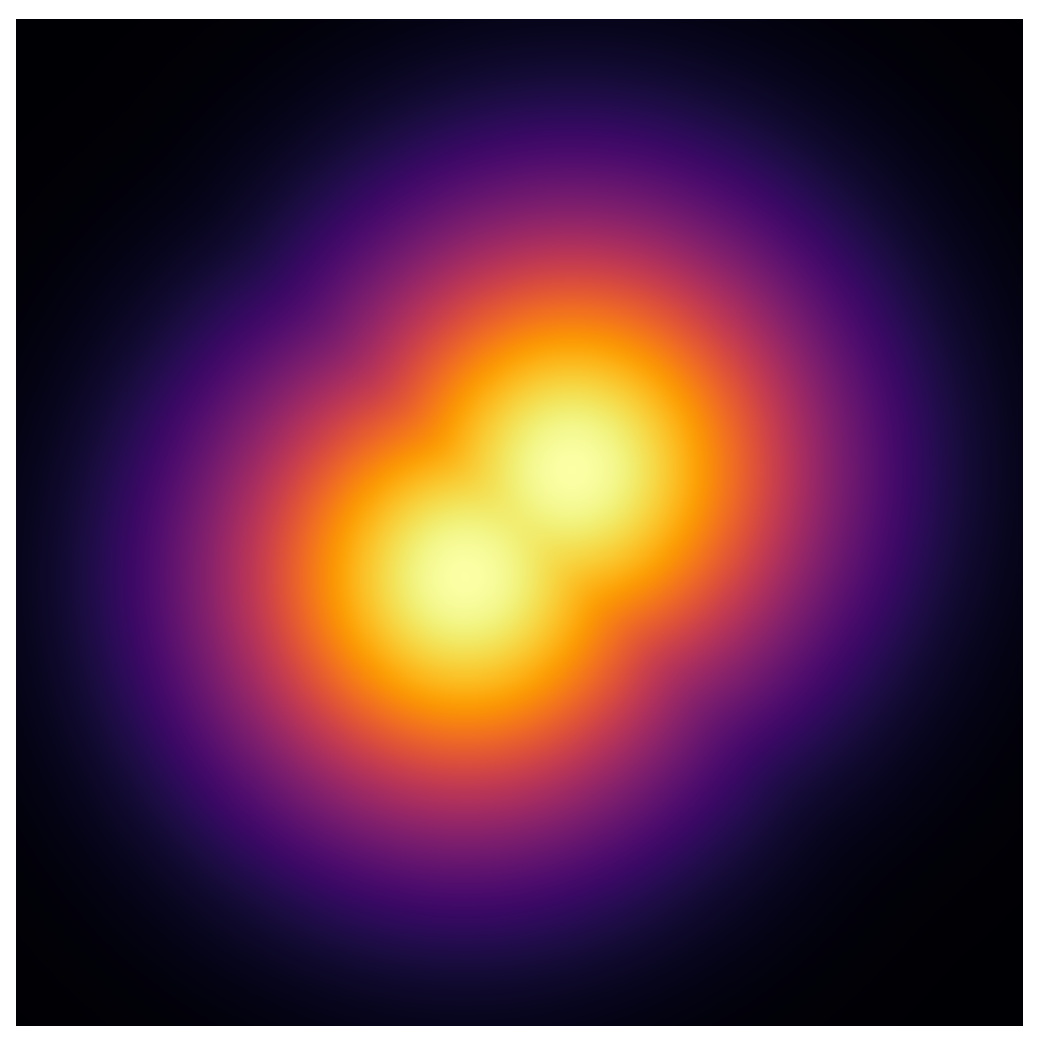
\includegraphics[width=\linewidth]{../img/heatmap_path_2.pdf}
%      \caption*{$\pi_2$}
    \end{minipage}%
    \begin{minipage}{0.333\linewidth}
      \centering
      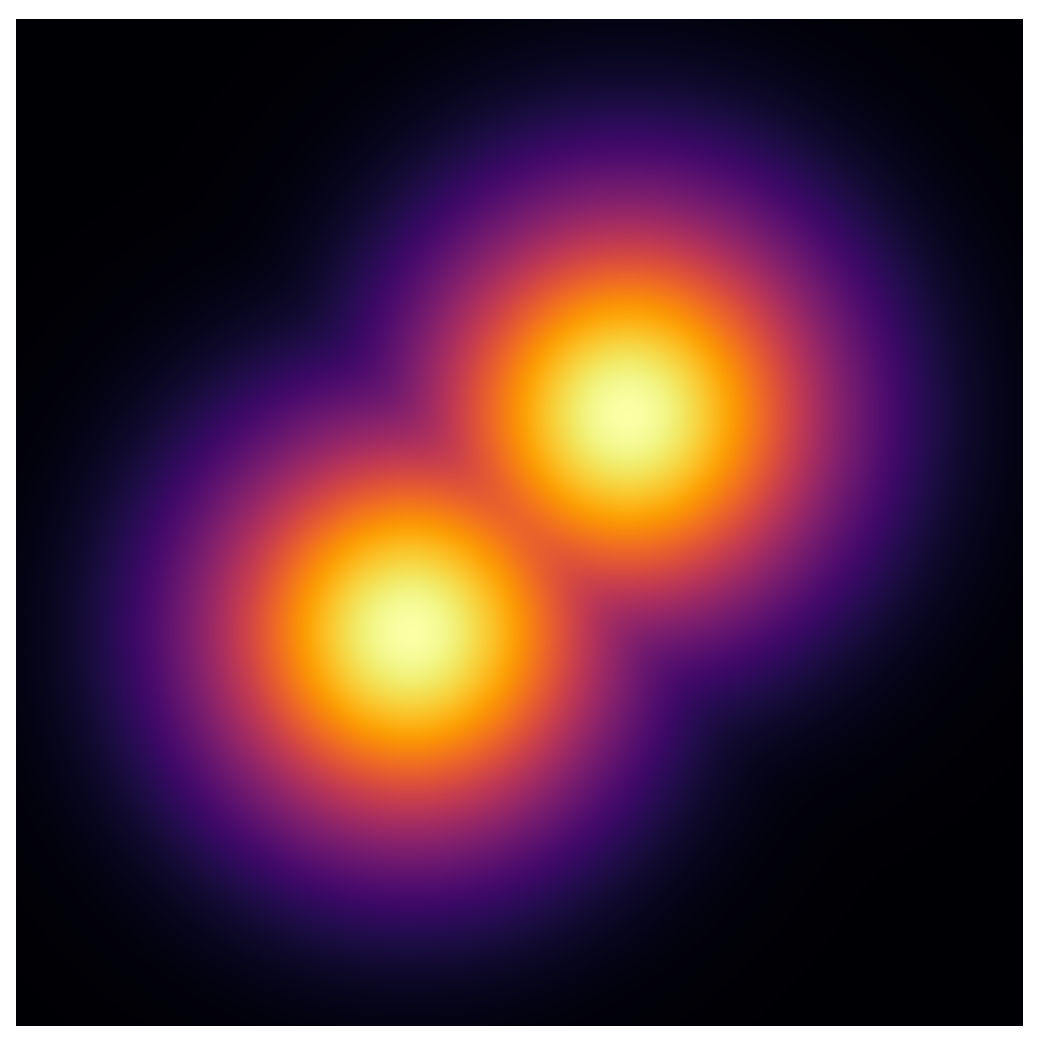
\includegraphics[width=\linewidth]{../img/heatmap_path_3.pdf}
%      \caption*{$\pi_3$}
    \end{minipage}\\
    \begin{minipage}{0.333\linewidth}
      \centering
      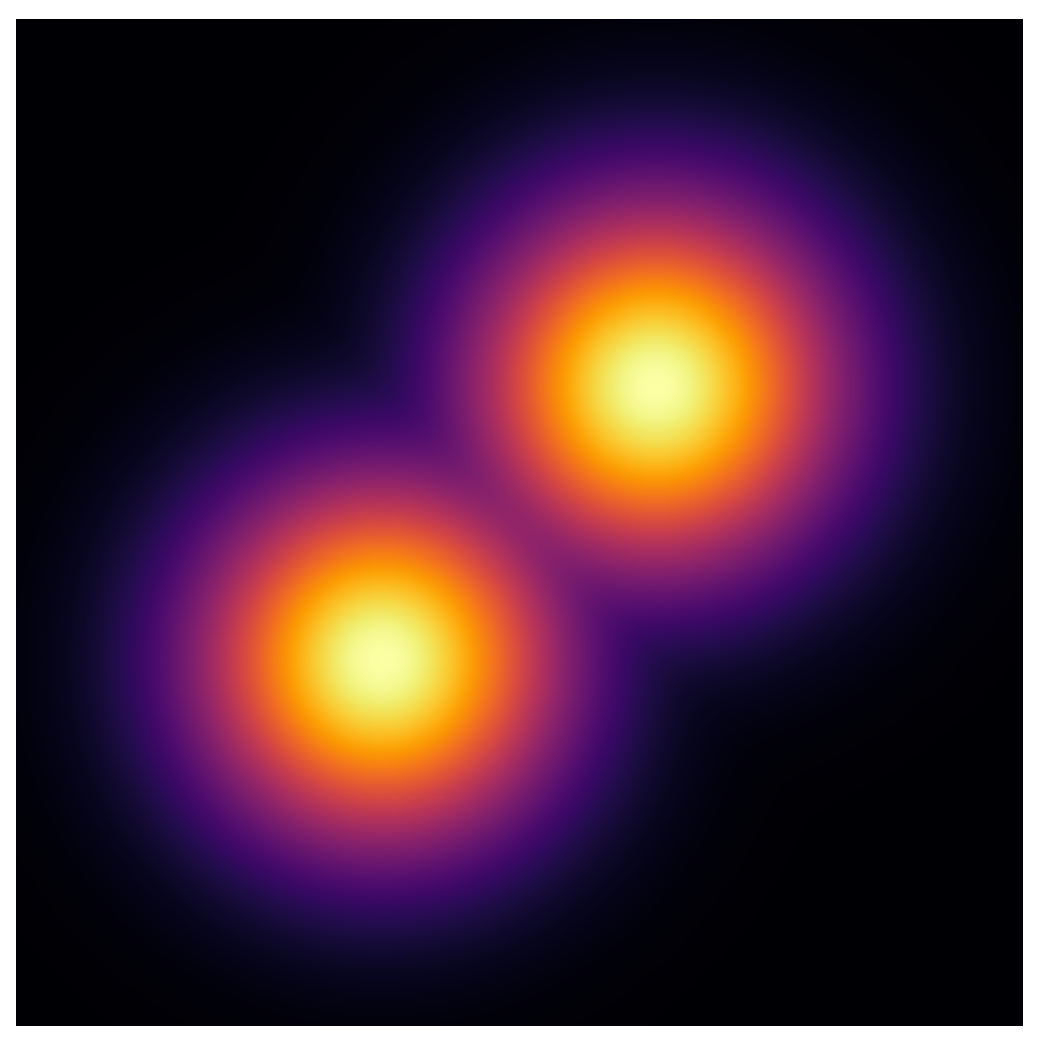
\includegraphics[width=\linewidth]{../img/heatmap_path_4.pdf}
%      \caption*{$\pi_4$}
    \end{minipage}%
    \begin{minipage}{0.333\linewidth}
      \centering
      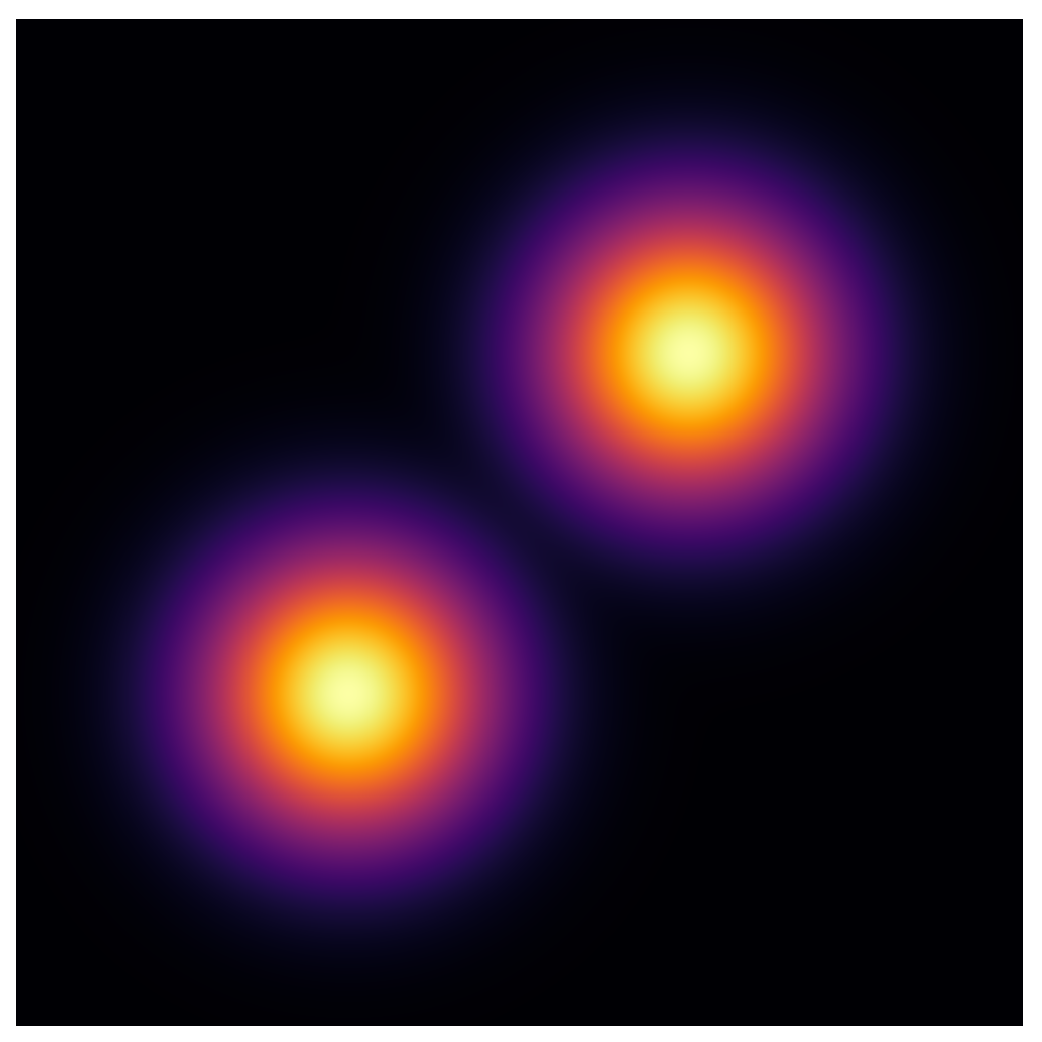
\includegraphics[width=\linewidth]{../img/heatmap_path_5.pdf}
%      \caption*{$\pi_5$}
    \end{minipage}%
    \begin{minipage}{0.333\linewidth}
      \centering
      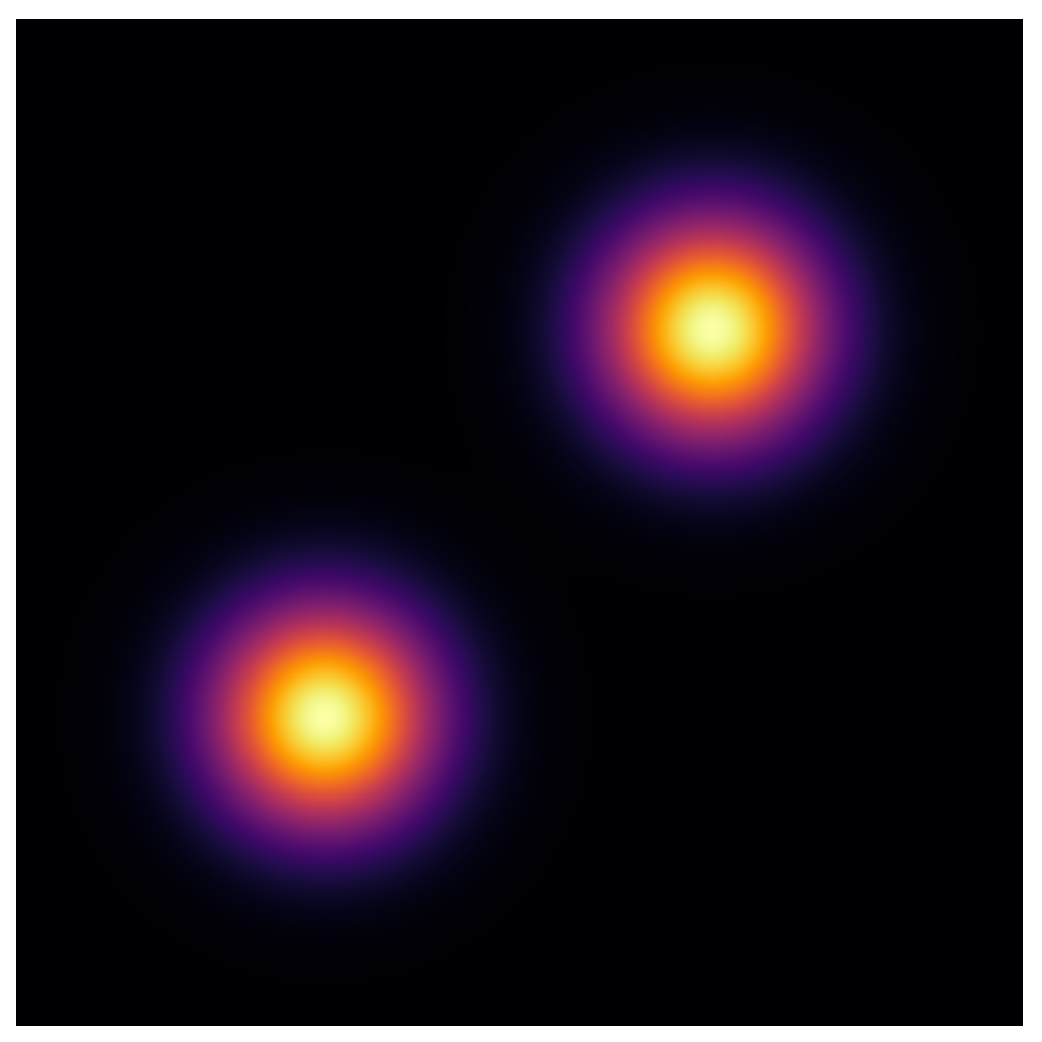
\includegraphics[width=\linewidth]{../img/heatmap_path_6.pdf}
%      \caption*{$\pi_6$}
    \end{minipage}
    \caption{Heatmaps of six distributions lying on an annealing path, 
    starting from a unimodal reference (top-left), and ending at a target
    distribution from \cref{fig:bimodal}.}
    \label{fig:path}
\end{figure}

To resolve this issue, PT constructs a sequence of $N$ distributions,  
$\pi_1, \pi_2, \ldots, \pi_N$, where $\pi_N$ is usually equal to the target $\pi$.
The distributions are chosen so that it is easy to obtain samples from $\pi_1$---%
called the \emph{reference} distribution---with the sampling difficulty increasing 
as one approaches $\pi_N$. An example of such a sequence of distributions, referred 
to as an \emph{annealing path}, is shown in \cref{fig:path}.

PT operates by first obtaining samples from each distribution on the path in parallel;
this is called an \emph{exploration} phase. Then, in the \emph{communication} phase, 
PT proposes swapping the samples between adjacent distributions. This step is crucial:
successive swaps along the path amount to transporting samples from the reference
to the target. This allows for the discovery of new regions of the space of the 
target distribution such as the top-right mode in \cref{fig:bimodal}.
